\documentclass[border=10pt]{standalone}
\usepackage{pgfplots}
\pgfplotsset{width=10cm,compat=1.8}
\begin{document}
\begin{tabular}{c}
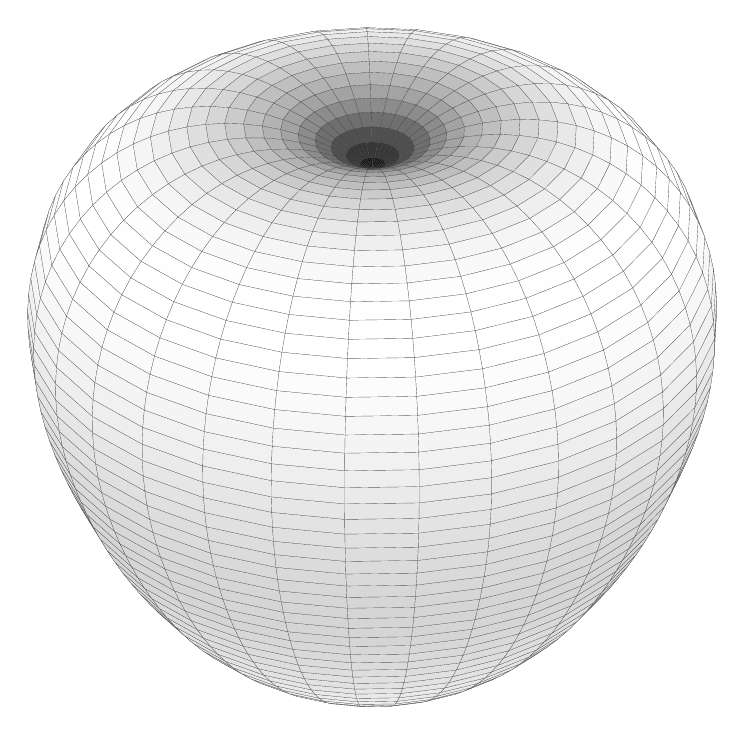
\begin{tikzpicture}
  \begin{axis}[
    hide axis,
    clip=false,
    y domain=0:180,
    samples=30,
    axis equal,
    view={45}{30},
    width=25cm,
    at={(0cm,0cm)},
    %colorbar,
    %colorbar/width=1cm,
    %colorbar horizontal,
    %colorbar style={
    %  height=1cm,
    %  yshift=-0.4cm,
    %  ytick={-1,1}
    %},
    colormap={iron}{[1pt]%
    rgb255(-1000pt)=(254,254,254),%%
rgb255(-968pt)=(254,254,254),%%
rgb255(-936pt)=(255,255,255),%%
rgb255(-905pt)=(255,255,255),%%
rgb255(-873pt)=(255,255,255),%%
rgb255(-841pt)=(254,254,254),%%
rgb255(-809pt)=(253,253,253),%%
rgb255(-777pt)=(251,251,251),%%
rgb255(-745pt)=(248,248,248),%%
rgb255(-714pt)=(245,245,245),%%
rgb255(-682pt)=(242,242,242),%%
rgb255(-650pt)=(238,238,238),%%
rgb255(-618pt)=(235,235,235),%%
rgb255(-586pt)=(233,233,233),%%
rgb255(-554pt)=(230,230,230),%%
rgb255(-523pt)=(227,227,227),%%
rgb255(-491pt)=(225,225,225),%%
rgb255(-459pt)=(222,222,222),%%
rgb255(-427pt)=(220,220,220),%%
rgb255(-395pt)=(217,217,217),%%
rgb255(-363pt)=(216,216,216),%%
rgb255(-332pt)=(214,214,214),%%
rgb255(-300pt)=(213,213,213),%%
rgb255(-268pt)=(213,213,213),%%
rgb255(-236pt)=(213,213,213),%%
rgb255(-204pt)=(213,213,213),%%
rgb255(-172pt)=(214,214,214),%%
rgb255(-141pt)=(215,215,215),%%
rgb255(-109pt)=(217,217,217),%%
rgb255(-77pt)=(219,219,219),%%
rgb255(-45pt)=(221,221,221),%%
rgb255(-13pt)=(224,224,224),%%
rgb255(19pt)=(227,227,227),%%
rgb255(50pt)=(230,230,230),%%
rgb255(82pt)=(233,233,233),%%
rgb255(114pt)=(237,237,237),%%
rgb255(146pt)=(240,240,240),%%
rgb255(178pt)=(243,243,243),%%
rgb255(210pt)=(246,246,246),%%
rgb255(241pt)=(249,249,249),%%
rgb255(273pt)=(252,252,252),%%
rgb255(305pt)=(253,253,253),%%
rgb255(337pt)=(255,255,255),%%
rgb255(369pt)=(255,255,255),%%
rgb255(401pt)=(255,255,255),%%
rgb255(432pt)=(254,254,254),%%
rgb255(464pt)=(252,252,252),%%
rgb255(496pt)=(248,248,248),%%
rgb255(528pt)=(244,244,244),%%
rgb255(560pt)=(238,238,238),%%
rgb255(592pt)=(231,231,231),%%
rgb255(623pt)=(223,223,223),%%
rgb255(655pt)=(214,214,214),%%
rgb255(687pt)=(204,204,204),%%
rgb255(719pt)=(193,193,193),%%
rgb255(751pt)=(181,181,181),%%
rgb255(783pt)=(167,167,167),%%
rgb255(814pt)=(148,148,148),%%
rgb255(846pt)=(122,122,122),%%
rgb255(878pt)=(91,91,91),%%
rgb255(910pt)=(63,63,63),%%
rgb255(942pt)=(44,44,44),%%
rgb255(974pt)=(0,0,0)%%
},
    point meta=atan(z/(sqrt(x^2+y^2)))
    ]

  \addplot3 [
      domain=0:360,
      surf,
      shader=flat,
      z buffer=sort,
      %fill=white!50!gray,
      draw=gray!50!black,
      line join=bevel,
      line width=0.002cm,
      samples y=60
    ]
    (
      {(1+exp(-(y/180*pi-pi/4)^2)+sin(y/2)+0.3*exp(-(y/180*pi-pi)^2))*sin(y)*cos(x)},
      {(1+exp(-(y/180*pi-pi/4)^2)+sin(y/2)+0.3*exp(-(y/180*pi-pi)^2))*sin(y)*sin(x)},
      {(1+exp(-(y/180*pi-pi/4)^2)+sin(y/2)+0.3*exp(-(y/180*pi-pi)^2))*cos(y)}
    );
    -- cycle;
   \end{axis}
\end{tikzpicture}
\\
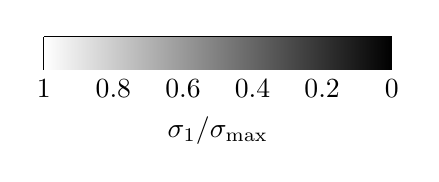
\begin{tikzpicture}
  %A-opt countour
\begin{axis}[%
view={0}{90},
shader=interp,
%3d box=complete,
grid=major,
xlabel = {$\sigma_1/\sigma_{\mathrm{max}}$},
xmin = 0, xmax = 1,
ymin = 0, ymax =1,
view/h=-180,
width=6cm,
height=2cm,
at={(9.5cm,4cm)},
    colormap={blackwhite}{[1cm] rgb255(0cm)=(0,0,0) rgb255(1cm)=(255,255,255)},
yticklabels={,,}
],

\addplot3[%
surf,
samples=30,
domain=0:1,
y domain=0:1,
]
{x};
\end{axis}
\end{tikzpicture}
\end{tabular}
\end{document}